\begin{chapter}{Redes Empregadas na Avaliação dos Modelos} \label{cap:lista-redes}
% select nme_network, to_char(s_score, '0.99'), n_vertices, n_edges 
% from view_network
% where fk_classification = 1
% OR nme_network ilike '%irpf%'
%
\begin{center}
\begin{longtable}{| p{10cm} | c | r | r |}
	\hline
	\textbf{Sistema} & \textbf{Valor} S & \textbf{Vértices} & \textbf{Arestas} \\ \hline
	\hline
	AbaGuiBuilder-1.8 &  $0,97$ & 2929 & 12399 \\ \hline
	alfresco-labs-deployment-3Stable &  $0,97$ & 2441 & 9178 \\ \hline
	aoi272 &  $0,98$ & 1579 & 11670 \\ \hline
	ArgoUML-0.28 &  $0,97$ & 5075 & 29018 \\ \hline
	battlefieldjava-0.1 &  $0,98$ & 707 & 2038 \\ \hline
	broker-4.1.5 &  $0,97$ & 5940 & 25589 \\ \hline
	checkstyle-5.0 &  $0,98$ & 1174 & 4513 \\ \hline
	dbwrench &  $0,98$ & 2015 & 10188 \\ \hline
	dom4j-1.6.1 &  $0,98$ & 4666 & 31689 \\ \hline
	ec2-api-tools &  $0,98$ & 5255 & 26916 \\ \hline
	ermodeller-1.9.2-binary &  $0,97$ & 1441 & 6261 \\ \hline
	findbugs-1.3.8 &  $0,98$ & 3401 & 20023 \\ \hline
	flyingsaucer-R8 &  $0,97$ & 1323 & 6610 \\ \hline
	freetts-1.2.2-bin &  $0,91$ & 273 & 1106 \\ \hline
	ganttproject-2.0.9 &  $0,98$ & 5447 & 25558 \\ \hline
	gdata-src.java-1.31.1 &  $0,97$ & 1649 & 8150 \\ \hline
	GEF-0.13-bin &  $0,97$ & 352 & 1484 \\ \hline
	geoserver-2.0-beta1-bin &  $0,97$ & 25007 & 145034 \\ \hline
	geotools-2.5.5-bin &  $0,97$ & 13559 & 79499 \\ \hline
	gfp\_0.8.1 &  $0,87$ & 475 & 1030 \\ \hline
	guice-2.0 &  $0,98$ & 638 & 2980 \\ \hline
	gwt-windows-1.6.4 &  $0,98$ & 6065 & 32729 \\ \hline
	hibernate-distribution-3.3.1.GA-dist &  $0,98$ & 4340 & 22410 \\ \hline
	Hl7Comm.1.0.1 &  $0,97$ & 337 & 1335 \\ \hline
	hsqldb\_1\_8\_0\_10 &  $0,95$ & 369 & 1901 \\ \hline
	iBATIS\_DBL-2.1.5.582 &  $0,95$ & 291 & 1300 \\ \hline
	iFreeBudget-2.0.9 &  $0,98$ & 4053 & 20028 \\ \hline
	iReport-nb-3.5.1 &  $0,97$ & 35019 & 184701 \\ \hline
	IRPF2009v1.1 &  $0,98$ & 5396 & 29247 \\ \hline
	JabRef-2.5b2-src &  $0,98$ & 2473 & 10437 \\ \hline
	jai-1\_1\_4-pre-dr-b03-lib-linux-i586 &  $0,96$ & 936 & 5086 \\ \hline
	jailer\_2.9.9 &  $0,97$ & 3691 & 14890 \\ \hline
	jakarta-tomcat-5.0.28-embed &  $0,98$ & 2314 & 10652 \\ \hline
	jalopy-1.5rc3 &  $0,98$ & 888 & 4349 \\ \hline
	jasperreports-3.5.2-project &  $0,98$ & 20508 & 120243 \\ \hline
	jfreechart-1.0.13 &  $0,97$ & 1989 & 13891 \\ \hline
	jGnash-2.2.0 &  $0,98$ & 6948 & 38303 \\ \hline
	jgraphpad-5.10.0.2 &  $0,96$ & 519 & 2257 \\ \hline
	jmsn-0.9.9b2 &  $0,83$ & 232 & 777 \\ \hline
	juel-2.1.2 &  $0,94$ & 111 & 435 \\ \hline
	juxy-0.8 &  $0,97$ & 3025 & 20427 \\ \hline
	JXv3.2rc2deploy &  $0,96$ & 711 & 2573 \\ \hline
	makagiga-3.4 &  $0,98$ & 1999 & 10819 \\ \hline
	MegaMek-v0.34.3 &  $0,98$ & 2855 & 19575 \\ \hline
	mondrian-3.1.1.12687 &  $0,97$ & 2000 & 14128 \\ \hline
	myjgui\_0.6.6 &  $0,96$ & 604 & 2430 \\ \hline
	oddjob-0.26.0 &  $0,98$ & 4204 & 18752 \\ \hline
	openxava-3.1.2 &  $0,98$ & 16919 & 89049 \\ \hline
	pdfsam-1.1.3-out &  $0,97$ & 3043 & 16024 \\ \hline
	peer-4.1.5 &  $0,97$ & 9291 & 50614 \\ \hline
	pentaho-reporting-engine-classic-0.8.9.11 &  $0,98$ & 3454 & 17948 \\ \hline
	pjirc\_2\_2\_1\_bin &  $0,84$ & 180 & 687 \\ \hline
	pmd-bin-4.2.5 &  $0,98$ & 1719 & 8098 \\ \hline
	proguard4.3 &  $0,98$ & 604 & 4923 \\ \hline
	rapidminer-4.4-community &  $0,96$ & 11764 & 55976 \\ \hline
	smc\_6\_0\_0 &  $0,97$ & 698 & 3571 \\ \hline
	squirrel-sql-3.0.1-base &  $0,98$ & 8982 & 43806 \\ \hline
	squirrel-sql-3.0.1-standard &  $0,98$ & 11922 & 53969 \\ \hline
	stendhal-0.74 &  $0,97$ & 747 & 3056 \\ \hline
	subethasmtp-3.1 &  $0,98$ & 1485 & 8174 \\ \hline
	thinkui\_sqlclient-1.1.2 &  $0,97$ & 2883 & 21979 \\ \hline
	tvbrowser-2.7.3-bin &  $0,97$ & 3335 & 14110 \\ \hline
	villonanny-2.3.0.b02.bin &  $0,98$ & 1949 & 6708 \\ \hline
	worker-4.1.5 &  $0,97$ & 5940 & 25589 \\ \hline
	zk-bin-3.6.1 &  $0,95$ & 13911 & 82219 \\ \hline
	
	\caption{\label{tab:redes}Sistemas de software usados no estudo de software-realismo de modelos e respectivos valores S.}
\end{longtable}
\end{center}


\begin{center}
\begin{longtable}{| p{6cm} | l | r | r | }
	\hline
	\textbf{Rede} & \textbf{Valor} S & \textbf{Vértices} & \textbf{Arestas} \\ \hline
	\hline
	5 redes de amizade do site Facebook \cite{Traud2008} & $-0,130 \pm 0,007$ & 768 a 18162 & 33312 a 1533600 \\ \hline
	3 redes de circuitos eletrônicos \cite{Milo2004} & $0,433 \pm 0,005$ & 121 a 511 & 189 a 819 \\ \hline
	4 redes de adjacências entre palavras \cite{Milo2004} & $0,573 \pm 0,064$ & 2703 a 11585 & 8300 a 46281 \\ \hline
	3 redes de estrutura proteica \cite{Milo2004} & $0,540 \pm 0,046$ & 52 a 96 & 123 a 213 \\ \hline
	2 redes sociais de sentimento positivo \cite{Milo2004} & $0,555 \pm 0,248$ & 31 a 66 & 96 a 182 \\ \hline
	43 redes metabólicas \cite{Jeong2000} & $0,509 \pm 0,015$ & 408 a 2360 & 792 a 5959 \\ \hline
	Rede de interação entre proteínas da levedura \cite{Jeong2001} & $0,22$ & 687 & 1079 \\ \hline
	Links entre blogs políticos \cite{Adamic2005} & $0,96$ & 1489 & 19090 \\ \hline
	Rede neural do verme C Elegans \cite{Watts1998} & $0,87$ & 296 & 2359 \\ \hline
	Rede ``beta3sreduced'' (fonte desconhecida) & $0,05$ & 1286 & 33813 \\ \hline
	Rede ``czech'' (fonte desconhecida) & $0,78$ & 5225 & 51687 \\  \hline
	Rede ``ecoli-metabolic'' (fonte desconhecida) & $0,69$ & 895 & 964 \\ \hline
	
	\caption{\label{tab:redes-outros}Redes de domínios diversos usados no estudo de software-realismo de modelos e respectivos valores S.}
\end{longtable}
\end{center}

\end{chapter}

\begin{chapter}{Algoritmos de Agrupamento} \label{cap:agrupamento}

A seguir são descritos brevemente três tipos de algoritmos de agrupamento de software que operam sobre redes de dependências entre entidades. % Para esta pesquisa foram escolhidos algoritmos estudados por diferentes grupos de pesquisa e com implementações disponíveis publicamente.

\begin{section}{Algoritmos Hierárquicos Aglomerativos}

Algoritmos hierárquicos aglomerativos têm sido aplicados a diversos problemas, incluindo o agrupamento de software \cite{Anquetil1999,Maqbool2007}. Essa família de algoritmos funciona com qualquer descrição de entidade, desde que seja fornecida uma métrica de similaridade entre pares de entidades. A similaridade entre duas entidades é medida em uma escala contínua de 0 a 1. O algoritmo é simples: inicia-se com um módulo para cada entidade e então mesclam-se sucessivamente os dois módulos mais similares até restar apenas um módulo com todas as entidades.

No contexto de recuperação de arquitetura de software, é comum descrever as entidades de código-fonte como um grafo de dependências entre entidades e usar a métrica de Jaccard para medir a similaridade entre duas entidades \cite{Anquetil1999}. Sejam X e Y duas entidades, e seja d(A) o conjunto de entidades ligadas à entidade A no grafo de dependências. A similaridade entre duas entidades, X e Y, é dada pela expressão a seguir:

$$
\mathrm{sim}(X, Y) ~=~ \frac{|\mathrm{d}(X) \cap \mathrm{d}(Y)|}{|\mathrm{d}(X) \cup \mathrm{d}(Y)|}
$$

O que diferencia os algoritmos hierárquicos aglomerativos entre si é o critério usado para medir a similaridade entre dois módulos. Os dois critérios mais estudados no contexto de agrupamento são chamados de ligação simples (SL, do inglês \emph{single linkage}) e ligação completa (CL, do inglês \emph{complete linkage}). Na ligação simples, a similaridade entre dois módulos é computada como a maior similaridade entre pares de entidades tiradas uma de cada módulo. Na ligação completa é considerada a menor similaridade.

Naturalmente, um agrupamento que consiste de apenas um módulo com todas as entidades analisadas é de pouco valor. Por essa razão deve existir um critério de parada que interrompa o algoritmo antes de todos os módulos terem sido mesclados em um grande módulo. No contexto de agrupamento de software, o critério mais comumente usado é a altura de corte, $h$, que varia entre 0 e 1. Sob esse critério, o algoritmo interrompe sua execução quando a maior similaridade entre dois módulos é menor ou igual a $1 - h$. Assim, quanto maior a altura de corte $h$, menor o número de módulos do agrupamento resultante.
	
\end{section}

\begin{section}{Bunch}

Com a finalidade de auxiliar a compreensão de programas, o algoritmo Bunch \cite{Mancoridis1998} agrupa o conjunto de entidades de um programa de acordo com os relacionamentos existentes entre elas, representados como um grafo orientado. O agrupamento é tratado como um problema de otimização no qual o objetivo é maximizar uma função denominada qualidade de modularização (QM), que recompensa agrupamentos com muitas arestas internas (que ligam entidades de um mesmo módulo) e poucas arestas externas (que ligam entidades de módulos distintos).

% TODO: fórmula da QM

Encontrar um agrupamento que possui QM ótima é um problema intratável; por isso o algoritmo Bunch usa heurísticas como algoritmos genéticos e \emph{hill-climbing} para obter resultados quase ótimos.

\end{section}

\begin{section}{ACDC}

O algoritmo ACDC \cite{Tzerpos2000} foi projetado com o intuito de encontrar agrupamentos que facilitam a compreensão de programas. Assim como o Bunch, ele opera sobre grafos orientados. Sua principal característica é a identificação de conjuntos dominantes de vértices no grafo. Um conjunto dominante é um conjunto de vértices, $v_0, v_1, \ldots{}, v_n$, onde $v_0$ é o vértice dominante, que satisfaz a duas condições: (i) existe um caminho entre $v_0$ e qualquer $v_i$; (ii) qualquer caminho de um vértice que não pertence ao conjunto até um vértice do conjunto, $v_i$, passa por $v_0$. O algoritmo ACDC identifica os conjuntos dominantes, em ordem crescente de número de vértices, e considera-os módulos do agrupamento. 

% subgraph dominator
% evita módulos muito grandes.
	
\end{section}	

\end{chapter}


% \begin{chapter}{Métrica MoJoSim} \label{cap:mojosim}
% 
% A métrica MoJoSim \cite{Bittencourt2009}, baseada na métrica MoJo \cite{Tzerpos1999}, mede a similaridade entre dois agrupamentos, um dos quais é considerado agrupamento de referência. Neste capítulo a métrica MoJo é explicada através de um exemplo e, a seguir, a métrica MoJoSim é definida.
% 
% % TODO: reescrever sem emoção, afinal isto virou um apêndice. Talvez mover o início para o capítulo do estudo.
% 
% % Como já foi mencionado, não existe um critério objetivo para determinar qual é o melhor agrupamento das entidades de um sistema de software. Ainda assim, alguma forma de avaliação de algoritmos de agrupamento é necessária para comparar os diferentes algoritmos. Uma das formas de avaliar os agrupamentos produzidos por algoritmos comparando-os com agrupamentos de referência, produzidos por especialistas, do conjunto de sistemas nos quais os algoritmos foram executados \cite{Koschke2000}.
% 
% A Figura \ref{fig:mojo} ilustra dois agrupamentos de um mesmo sistema de software hipotético, representado como um grafo orientado que descreve dependências estáticas entre classes do sistema. É fácil perceber que os agrupamentos não são idênticos: um deles possui quatro módulos, enquanto o outro possui três. Ainda assim, os agrupamentos são bastante semelhantes. O módulo $M_4$ corresponde exatamente ao módulo $M_C$; O módulo $M_3$ é quase igual ao módulo $M_B$; e os módulos $M_1$ e $M_2$, unidos, são parecidos com o módulo $M_A$.
% 
% \begin{figure}[htbp]
% 	\centering
% 		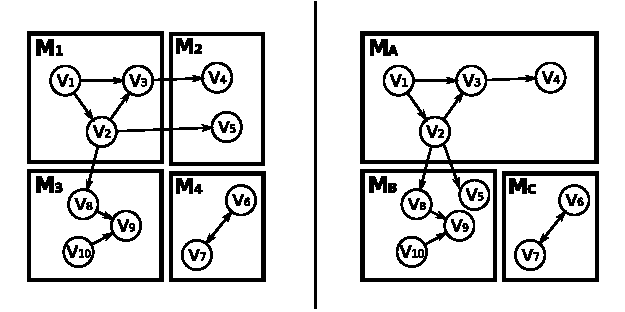
\includegraphics[scale=1]{figuras/redes-dupla}
% 	\caption{Dois agrupamentos de um mesmo sistema de software hipotético, descrito como um grafo que representa dependências entre classes.}
% 	\label{fig:mojo}
% \end{figure}
% 
% % É fácil verificar se dois agrupamentos de um mesmo conjunto de entidades são idênticos ou não. Para comparar diferentes agrupamentos produzidos por algoritmos, no entanto, é preciso definir uma métrica de similaridade entre agrupamentos que seja capaz de determinar qual agrupamento de uma coleção de agrupamentos é mais similar a um agrupamento de referência.
% 
% A ideia por trás da métrica MoJo é que um agrupamento dado é muito similar a um agrupamento de referência se é possível transformar o primeiro agrupamento no segundo usando poucas operações do tipo mover e mesclar. A operação mover consiste de mover uma entidade de um módulo para outro módulo distinto. A operação mesclar consiste de mesclar dois módulos. O MoJo entre  dois agrupamentos é igual ao número de operações de mover e mesclar que são necessárias para transformar o primeiro agrupamento no segundo. Quanto menor o MoJo, maior a similaridade entre dois agrupamentos; agrupamentos idênticos têm MoJo igual a zero.
% 
% % A métrica MoJo não é simétrica. Para chegar a essa conclusão, basta observar que há uma operação de mesclar módulos, mas não uma operação de dividir um módulo em dois. No contexto de avaliação de algoritmos de agrupamento de software, é considerado o número de operações necessárias para transformar o agrupamento encontrado por um algoritmo no agrupamento de referência, e não o contrário.
% 
% Na Figura \ref{fig:mojo}, considerando que o agrupamento de referência é o segundo (o da direita), o MoJo entre os dois agrupamentos vale 2. Para transformar o primeiro agrupamento no segundo são necessárias, portanto, duas operações: mesclar os módulos $M_1$ e $M_2$, e mover o vértice $v_5$ para o módulo $M_3$. Após a realização dessas operações, os agrupamentos se tornam idênticos, considerando as correspondências $(M_1 \cup M_2) = M_A$, $M_3 = M_B$ e $M_4 = M_C$.
% 
% Observando que o valor MoJo entre dois agrupamentos com o mesmo número de entidades varia entre 0 e o número de entidades em cada agrupamento, $n$, é possível definir uma métrica, chamada MoJoSim, que mapeia o valor MoJo em uma escala de 0 a 1 \cite{Bittencourt2009}. O valor 0 representa a menor similaridade e o valor 1, a maior similaridade. O valor de MoJoSim entre dois agrupamentos é definido de acordo com a seguinte equação:
% 
% $$
% \mathrm{MoJoSim}(X, Y) ~=~ 1 - \frac{\mathrm{MoJo}(X, Y)}{n}
% $$
% 
% O valor de MoJoSim na Figura \ref{fig:mojo} é, portanto, igual a $1 - \frac{2}{10} = 0,8$.
% 
% % Anquetil avaliou 
% 
% % Movido
% % Wu, Hassan e Holt \cite{Wu2005} avaliaram os algoritmos Bunch, ACDC e algoritmos aglomerativos comparando, através da métrica MoJo, os agrupamentos encontrados pelos algoritmos com agrupamentos de referência de 5 sistemas de software em C e C++, representados como um grafo dos arquivos fonte e dependências estáticas entre os arquivos. Os agrupamentos de referência foram obtidos automaticamente a partir de uma análise da estrutura de diretórios dos sistemas. Cada diretório contendo pelo menos 5 arquivos fonte foi considerado um módulo do sistema. Bittencourt e Guerrero \cite{Bittencourt2009} realizaram um experimento semelhante, porém avaliando algoritmos de agrupamento estudados em outros domínios aplicados sobre um conjunto de 4 sistemas em Java.
% 
% \end{chapter}
